\documentclass[border=2pt]{standalone}
\usepackage{tikz}
\usetikzlibrary{chains,arrows.meta}

\begin{document}
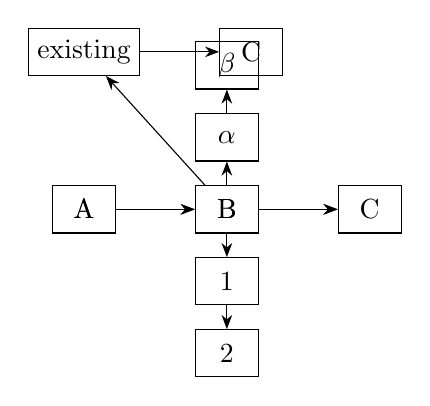
\begin{tikzpicture}[
  node distance=3mm and 10mm,
  every node/.style={draw, minimum width=8mm, minimum height=6mm},
  every join/.style={-{Stealth[length=1.8mm]}}
]
  % Adapted from the documented chains examples: chainin and delayed branches.
  \node (existing) at (0,2) {existing};
  \begin{scope}[start chain=walk going right]
    \node [on chain,join] {A};
    \node [on chain,join] (fork) {B};
    \chainin (existing) [join];
    \node [on chain,join] {C};
  \end{scope}

  \begin{scope}[start chain=trunk going right]
    \node [on chain,join] {A};
    \node [on chain,join] {B};
    \begin{scope}[start branch=numbers going below]\end{scope}
    \begin{scope}[start branch=greek going above]\end{scope}
    \node [on chain,join=with trunk/numbers-end,join=with trunk/greek-end] {C};
    \begin{scope}[continue branch=numbers]
      \node [on chain,join] {1};
      \node [on chain,join] {2};
    \end{scope}
    \begin{scope}[continue branch=greek]
      \node [on chain,join] {$\alpha$};
      \node [on chain,join] {$\beta$};
    \end{scope}
  \end{scope}
\end{tikzpicture}
\end{document}
